\chapter{Modelización hidrológica e hidráulica}
\label{ch:modelización}

\section{Rol de \hydra en la cadena metodológica}
\label{sec:rol_hydra}

\hydra no sustituye las metodologías hidrológicas, hidráulicas, climáticas o estadísticas existentes. Actúa como marco de integración capaz de coordinar estas metodologías dentro de una cadena de cálculo reproducible. Los motores de simulación conservan exactamente su comportamiento; los métodos estadísticos se invocan con las mismas formulaciones que en la literatura de referencia; los datos se obtienen de las mismas fuentes institucionales. La aportación de \hydra es la capa de orquestación que conecta cada uno de estos componentes, estandariza sus interfaces y los hace operables de forma conjunta.

La \cref{tab:componentes_hydra} resume los componentes de la cadena y las herramientas o metodologías que \hydra incorpora en cada bloque.

Este capítulo se centra en la parte física de la cadena: la transformación de escenarios climáticos, hidrológicos o sintéticos en respuestas de caudal, calado, velocidad y extensión inundada. En una metodología estocástica, esta transformación no puede hacerse manualmente caso a caso. Cada escenario debe generar entradas de modelo, ejecutarse con una configuración controlada y producir salidas comparables. El bloque de modelización existe precisamente para convertir modelos profesionales ya aceptados en piezas de una cadena repetible.

\begin{table}[htbp]
  \centering
  \caption{Componentes de la cadena metodológica de \hydra y herramientas o metodologías incorporadas.}
  \label{tab:componentes_hydra}
  \begin{tabular}{p{0.30\textwidth}p{0.60\textwidth}}
    \toprule
    Componente & Herramienta o metodología \\
    \midrule
    Fuentes de datos & ERA5, GPM/IMERG, PERSIANN, AEMET, OGIMET, Meteostat, GloFAS, GRDC, USGS, SoilGrids \\[3pt]
    Análisis de extremos & GEV/GPD · L-momentos · Inferencia bayesiana (PyMC, PyStan opcional) \\[3pt]
    Análisis multivariante & Cópulas gaussianas · Vine cópulas \\[3pt]
    Generación estocástica & NEOPRENE (NSRP puntual y STNSRP multisitio) · CoSMoS \\[3pt]
    Cambio climático & CMIP6 (CDS/ESGF) bajo escenarios SSP \\[3pt]
    Corrección de sesgo & Delta method · Quantile mapping \\[3pt]
    Downscaling híbrido & MaxDiss · k-NN \\[3pt]
    Emulación & Gaussian Process Regression (GPR) \\[3pt]
    Modelización hidrológica & HEC-HMS · SWAT \\[3pt]
    Modelización hidráulica & SFINCS · HEC-RAS · Iber \\[3pt]
    \bottomrule
  \end{tabular}
\end{table}

En ningún caso \hydra propone estas metodologías como contribuciones nuevas: las implementa, las conecta y las hace operables de forma conjunta. Su contribución reside en que esa integración, antes inexistente o dependiente de flujos manuales frágiles, es ahora reproducible, auditable y transferible a nuevos casos sin reconstruir la cadena desde cero.

\section{Objetivo del bloque}

El bloque de modelización conecta los datos y escenarios generados por \hydra con modelos físicos ampliamente utilizados en ingeniería hidrológica e hidráulica. Su objetivo es reducir la carga manual asociada a la configuración, ejecución por lotes y postprocesado de resultados, sin reemplazar los motores físicos ni modificar su comportamiento.

La arquitectura del bloque sigue el patrón de adaptador. Cada módulo traduce estructuras de datos internas de \hydra al formato esperado por el modelo externo, lanza la ejecución y transforma las salidas a productos comunes: hidrogramas como \texttt{pandas.Series}, mapas de calado como \texttt{xarray.DataArray}, y tablas de resultados como \texttt{pandas.DataFrame}. Esta estrategia mantiene la independencia entre \hydra y los motores físicos: cuando aparece una nueva versión del modelo o un nuevo motor alternativo, solo es necesario actualizar el adaptador correspondiente.

El patrón de adaptador tiene cuatro responsabilidades concretas. Primero, preparar entradas: escribir ficheros de precipitación, caudal, condiciones de contorno o parámetros en el formato nativo de cada motor. Segundo, ejecutar: lanzar el motor mediante API, controlador externo o subproceso, registrando versión, ruta de ejecutable y código de salida. Tercero, leer resultados: convertir DSS, HDF, NetCDF, GeoTIFF o ficheros de texto en estructuras comunes. Cuarto, validar: comprobar que la simulación terminó, que existen salidas esperadas y que los valores tienen unidades y rangos plausibles. Esta separación evita que el análisis estadístico dependa de formatos propietarios.

La integración tiene también límites explícitos. HYDRA no calibra automáticamente cualquier modelo por el hecho de ejecutarlo; solo automatiza las operaciones implementadas y documentadas en cada adaptador. Tampoco sustituye la revisión hidráulica experta: la estabilidad numérica, la calidad del MDT, la rugosidad, las condiciones de contorno y la representación de estructuras siguen siendo decisiones técnicas del modelo físico.

\section{Modelos hidrológicos}

\subsection{HEC-HMS}

HEC-HMS \parencite{scharffenberg2016hechms} es el modelo de simulación hidrológica del Cuerpo de Ingenieros del Ejército de los Estados Unidos. Simula procesos de precipitación-escorrentía a escala de cuenca, integrando métodos de pérdidas, transformación precipitación-caudal y propagación en cauces. Su uso está muy extendido en administraciones hidráulicas españolas, lo que lo convierte en el motor hidrológico preferente para estudios integrados con planes de zona inundable.

En la cadena de \pyhydra, HEC-HMS ocupa el papel de traductor entre lluvia y caudal. Es especialmente útil en casos como Calle 30, donde el forzamiento estocástico se genera como precipitación multisitio y debe convertirse en hidrogramas de entrada para el modelo hidráulico. Esta separación permite mantener el análisis estadístico de lluvia en el bloque climático y la respuesta de cuenca en un motor hidrológico reconocido.

El módulo \texttt{modeling.hydrology.hec\_hms} encapsula el acceso a HEC-HMS a través de tres funcionalidades:

\begin{description}
  \item[Preparación de entradas.] Las funciones \texttt{generate\_gage} y \texttt{fill\_gage\_series} escriben las series de precipitación o caudal en formato DSS mediante \texttt{hecdss} (independiente de la versión de \texttt{numpy}, a diferencia de \texttt{pydsstools}); \texttt{generate\_met} y \texttt{generate\_hms} actualizan respectivamente el modelo meteorológico y la estructura principal del proyecto para enlazar pluviómetros, cuenca, control y ejecución.

  \item[Ejecución.] La función \texttt{run\_hms\_script} lanza HEC-HMS en modo batch mediante un script generado automáticamente (API Jython en Windows, \texttt{xvfb-run} en Linux) y espera a su finalización; \texttt{read\_hms\_dss\_timeseries} lee después las series de salida del DSS resultante. La clase \texttt{HMSModel} envuelve este ciclo completo: su método \texttt{.run\_hms(*params)} ejecuta el modelo con un vector de parámetros y devuelve el caudal simulado como \texttt{ndarray}, delegando en \texttt{run\_hms\_script} y en la lectura DSS. Este patrón admite la ejecución de múltiples simulaciones en bucle, lo que permite la simulación sistemática del conjunto de eventos estocásticos.

  \item[Calibración automática con spotpy.] \texttt{HMSModel} por sí sola no calibra: expone la interfaz de ejecución (\texttt{.run\_hms(*params)}, punto de extensión \texttt{.\_write\_params(params)}) que hace de ella una \emph{setup class} compatible con \texttt{spotpy} \parencite{houska2015spotpy}. Su subclase \texttt{TextBasinHMSCalibrationModel} implementa esa escritura de parámetros editando directamente el fichero \texttt{.basin} como factores multiplicativos sobre valores base. La función \texttt{calibrate\_hms\_sceua} invoca internamente el algoritmo SCE-UA (\emph{shuffled complex evolution}) de \texttt{spotpy} sobre un \texttt{TextBasinHMSCalibrationModel}, con la función objetivo (NSE, PBIAS o RMSE) configurable. La integración actual cubre SCE-UA; otros algoritmos de \texttt{spotpy} (PSO, DREAM, etc.) son utilizables sobre la misma \emph{setup class} pero no están envueltos en una función dedicada de \pyhydra.
\end{description}

La calibración automática fue especialmente relevante en el estudio de los países andinos \parencite{paz2019idb,deljesus2020andinos}, donde la escala territorial y el número de cuencas hizo inviable la calibración manual de los modelos hidrológicos. La integración de esa experiencia en \hydra generaliza la capacidad a cualquier proyecto que use HEC-HMS como motor hidrológico.

\subsection{SWAT}

SWAT \parencite{arnold1998swat,gassman2007swat} es un modelo hidrológico semidistribuido de simulación continua, desarrollado por el USDA-ARS. A diferencia de HEC-HMS, que opera a escala de evento, SWAT simula el ciclo hidrológico completo con paso diario durante períodos de años o décadas, lo que lo hace adecuado para evaluación de recursos hídricos, análisis de tendencias y escenarios de cambio climático a largo plazo.

Por esa razón, SWAT se conecta principalmente con el bloque de cambio climático. Las series históricas y futuras corregidas por sesgo se transforman en entradas meteorológicas continuas, se ejecutan por escenario y se comparan salidas agregadas como aportaciones mensuales, caudal medio o indicadores de sequía. El interés industrial no está solo en ejecutar SWAT, sino en repetir el mismo flujo sobre decenas de combinaciones modelo--escenario--horizonte sin perder trazabilidad.

El módulo \texttt{modeling.hydrology.swat} gestiona la integración mediante un conjunto de funciones, no una clase orientada a objetos:

\begin{description}
  \item[Preparación de entradas climáticas.] Las funciones \texttt{write\_precipitation\_file} y \texttt{write\_temperature\_file} convierten series de precipitación y temperatura (históricas o proyecciones CMIP6 corregidas) al formato clásico de ficheros \texttt{.pcp}/\texttt{.tmp} de SWAT a partir de coordenadas de estación y series diarias; \texttt{write\_swatplus\_precipitation\_files} y \texttt{write\_swatplus\_temperature\_files} generan el equivalente para SWAT+ (ficheros individuales por estación más el índice \texttt{pcp.cli}/\texttt{tmp.cli}); \texttt{edit\_file\_cio} ajusta el período de simulación en \texttt{file.cio}.

  \item[Ejecución por escenarios.] La función \texttt{run\_swat} lanza el ejecutable de SWAT+ en el directorio \texttt{TxtInOut} del proyecto y devuelve el código de salida del proceso.
\end{description}

La lectura de las salidas de SWAT (\texttt{output.rch}, \texttt{output.sub}) no está actualmente automatizada dentro de \pyhydra: se realiza de forma ad-hoc en cada caso de estudio, fuera del paquete. Completar un lector genérico de estos ficheros es trabajo pendiente (\cref{ch:conclusiones}).

SIMPCCe \parencite{navas2025simpce} es el ejemplo más directo de uso de SWAT dentro del ecosistema \hydra para análisis de aportaciones a embalses españoles bajo proyecciones CMIP6.

\section{Modelos hidráulicos}

\subsection{SFINCS}

SFINCS \parencite{leijnse2021sfincs} (Super-Fast INundation of CoastS) es un modelo hidráulico bidimensional de física reducida desarrollado por Deltares. Su formulación simplificada de las ecuaciones de Saint-Venant reduce drasticamente el tiempo de computo manteniendo una precisión aceptable para inundación urbana y costera, lo que lo convierte en el motor preferente para flujos estocásticos con alto número de escenarios.

La ventaja de SFINCS dentro de \hydra es su escalabilidad. Al usar mallas regulares o cuasi-regulares y ficheros de configuración simples, se presta bien a la generación automática de proyectos y a la ejecución masiva. Esto lo convierte en una opción adecuada para atlas nacionales, análisis de sensibilidad o cribados iniciales donde el número de escenarios pesa más que el detalle hidráulico local.

El módulo \texttt{modeling.hydraulic.sfincs} proporciona:
\begin{description}
  \item[\texttt{setup\_sfincs\_model}] Configura la malla de cálculo a partir de geometría de cuenca, modelo digital de elevaciones, puntos de entrada y series de caudal. Devuelve un objeto \texttt{SfincsModel} que se persiste en disco mediante \texttt{mod.write()}.

  \item[\texttt{run\_sfincs}] Ejecuta SFINCS para el proyecto configurado en un directorio de trabajo.

  \item[\texttt{write\_manning\_wl\_boundary}] Escribe una condición de contorno de nivel aguas abajo calculada mediante Manning y actualiza los ficheros \texttt{sfincs.bnd}, \texttt{sfincs.bzs} y \texttt{sfincs.inp}.
\end{description}

La lectura de resultados SFINCS se concentra actualmente en \path{modeling.hydraulic.sensitivity}, mediante \path{load_sfincs_ensemble}. Esta función lee la variable \path{hmax} de los ficheros \path{sfincs_map.nc} producidos por ejecuciones en lote, georreferencia las coordenadas del modelo y devuelve un \path{xarray.DataArray} con una dimensión de simulación. Esta separación refleja el uso operativo del módulo: \path{sfincs.py} prepara y ejecuta proyectos, mientras que \path{sensitivity.py} agrega y analiza ensembles de resultados.

\subsection{HEC-RAS}

HEC-RAS \parencite{brunner2016hecras} es la referencia profesional más extendida para modelización hidráulica 1D/2D en administraciones y consultoría española. La memoria del MITECO para cartografía de zonas inundables \parencite{marm2011guia} referencia HEC-RAS como herramienta principal, lo que hace que una fracción significativa de los modelos hidráulicos calibrados en España estén en este formato.

En \hydra, HEC-RAS cubre dos necesidades distintas. En modelos 1D, como Calle 30, permite representar redes de conducción, tramos canalizados o sistemas lineales donde la geometría hidráulica está definida por secciones y conectividad. En modelos 2D, como los análisis posteriores del Besaya, permite obtener campos espaciales de calado y velocidad comparables con SFINCS. El adaptador actual se centra en preparar escenarios, modificar ficheros de proyecto y lanzar ejecuciones; la extracción espacial de resultados 2D se realiza en los flujos de postproceso de los casos, pero no está expuesta como función pública independiente en \texttt{pyhydra.modeling.hydraulic.hec\_ras}.

El módulo \texttt{modeling.hydraulic.hec\_ras} automatiza cuatro operaciones:
\begin{description}
  \item[\texttt{modify\_unsteady\_file}] Actualiza el fichero de flujo no permanente de HEC-RAS con una nueva serie de caudal, permitiendo simular diferentes escenarios sin modificar manualmente el proyecto.

  \item[\texttt{modify\_plan\_file} y \texttt{modify\_project\_file}] Actualizan el plan y el proyecto para activar el nuevo fichero de flujo no permanente.

  \item[\texttt{create\_flow\_series}] Suaviza series de caudal mediante máximo móvil centrado antes de escribirlas como condición de contorno.

  \item[\texttt{run\_hec\_ras}] Lanza el plan activo de HEC-RAS mediante \texttt{rascontrol}, condicionado a disponer de una instalación local compatible.
\end{description}

Su uso en Calle 30 \parencite{navas2024calle30} y en desarrollos posteriores sobre el entorno del Besaya demuestra la viabilidad de la automatización incluso en proyectos de complejidad industrial. La limitación principal es que HEC-RAS no dispone de una API pública documentada y estable para todos los modos de control externo, por lo que la integración se basa en la modificación de ficheros de texto, la ejecución del ejecutable vía subproceso o controlador disponible y la lectura sistemática de salidas.

\subsection{Iber}

Iber \parencite{blade2014iber} es un modelo hidráulico bidimensional de superficie libre desarrollado por el CEDEX y la Universidad de A Coruña. Su integración en el flujo de trabajo de \hydra se limita en la versión actual a la preparación de entradas (hidrogramas de entrada en el formato de ficheros de texto de Iber) y a la lectura de resultados exportados a GeoTIFF desde la interfaz gráfica. No se ha implementado un adaptador de automatización completo porque Iber no dispone de una API de línea de comandos documentada que permita la ejecución en modo \textit{batch} sin interacción con la interfaz gráfica, lo que hace inviable su uso en flujos estocásticos con cientos o miles de simulaciones. Esta limitación es la razón técnica por la que HEC-RAS y SFINCS, que sí admiten ejecución automatizada mediante subproceso o controlador externo, sustituyeron progresivamente a Iber en los desarrollos posteriores. La integración parcial es coherente con su papel en los trabajos iniciales de la línea, especialmente el Besaya \parencite{navas2018besaya} y Mallorca \parencite{navas2019mallorca}, donde se empleó para las simulaciones individuales del subconjunto representativo antes de que los adaptadores de HEC-RAS y SFINCS estuvieran disponibles.

\section{Análisis de sensibilidad}
\label{sec:sensibilidad}

El módulo \texttt{modeling.hydraulic.sensitivity} proporciona herramientas para análisis de sensibilidad de parámetros hidráulicos (rugosidad de Manning, condiciones de contorno) mediante ejecuciones sistemáticas del modelo con variaciones paramétricas. Su desarrollo recoge funciones generales surgidas durante el análisis del río Besaya \parencite{navas2025roughness}, pero los notebooks empleados para preparar ese artículo constituyen material interno de investigación y no forman parte de los ejemplos de uso de \hydra.

El objetivo del módulo no es sustituir un estudio de incertidumbre completo, sino facilitar el muestreo y la comparación sistemática de respuestas hidráulicas. En el caso del Besaya, el parámetro analizado fue la rugosidad de Manning por clases de uso del suelo; en otros dominios podrían analizarse condiciones de contorno, niveles aguas abajo o parámetros de infiltración. La estructura común es siempre la misma: generar un ensemble de configuraciones, ejecutar el modelo, cargar resultados y resumir la variabilidad de las métricas de impacto.

Las \cref{fig:manning_distributions,fig:sensibilidad_manning} ilustran los resultados obtenidos en el análisis de sensibilidad de Manning sobre el caso del río Besaya. La \cref{fig:manning_distributions} contrasta los valores bibliográficos, las distribuciones ajustadas y las muestras Monte Carlo para nueve clases de uso del suelo. La \cref{fig:sensibilidad_manning} resume primero el ensemble de entradas y después la respuesta intramodelo de SFINCS y HEC-RAS.

\begin{figure}[htbp]
  \centering
  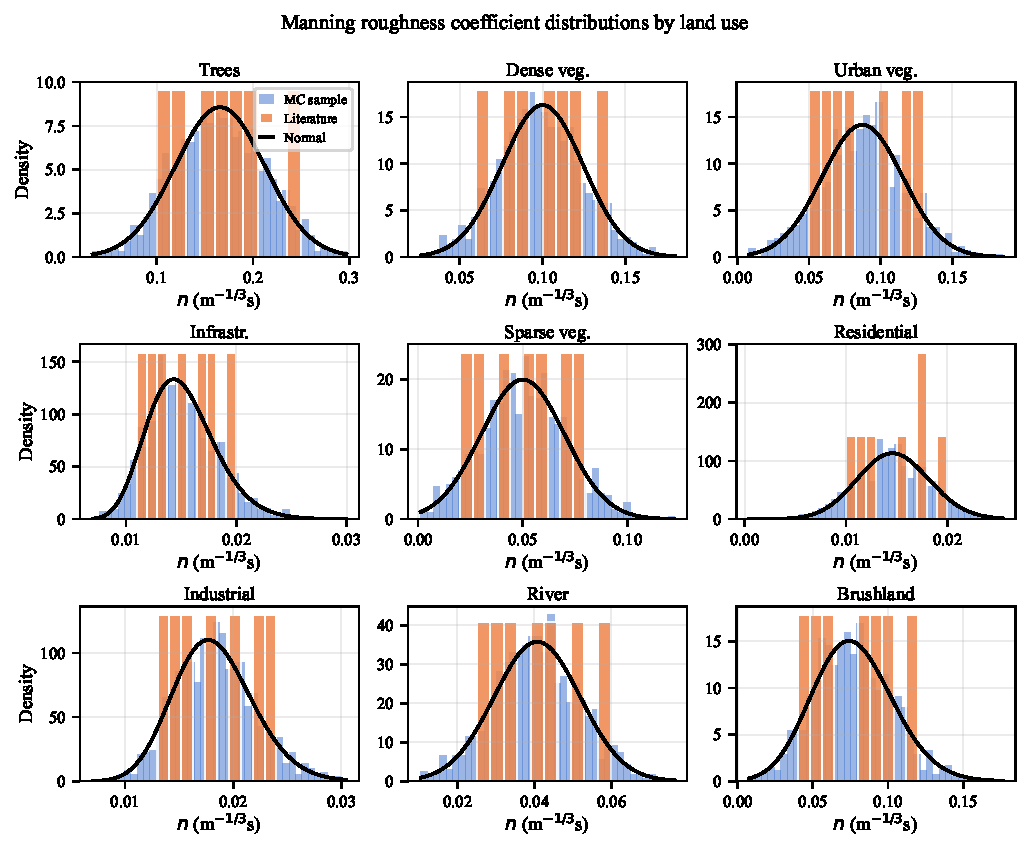
\includegraphics[width=0.75\textwidth]{figures/besaya_fig01_manning_distributions.pdf}
  \caption{Distribuciones ajustadas del coeficiente de Manning para nueve clases de uso del suelo en Los Corrales de Buelna. Los histogramas azules representan las 1.000 muestras Monte Carlo; las barras naranjas, los valores bibliográficos de referencia; y las curvas negras, la distribución seleccionada mediante el contraste de Kolmogorov--Smirnov. Fuente: \parencite{navas2025roughness}.}
  \label{fig:manning_distributions}
\end{figure}

\begin{figure}[htbp]
  \centering
  \begin{subfigure}[b]{0.48\textwidth}
    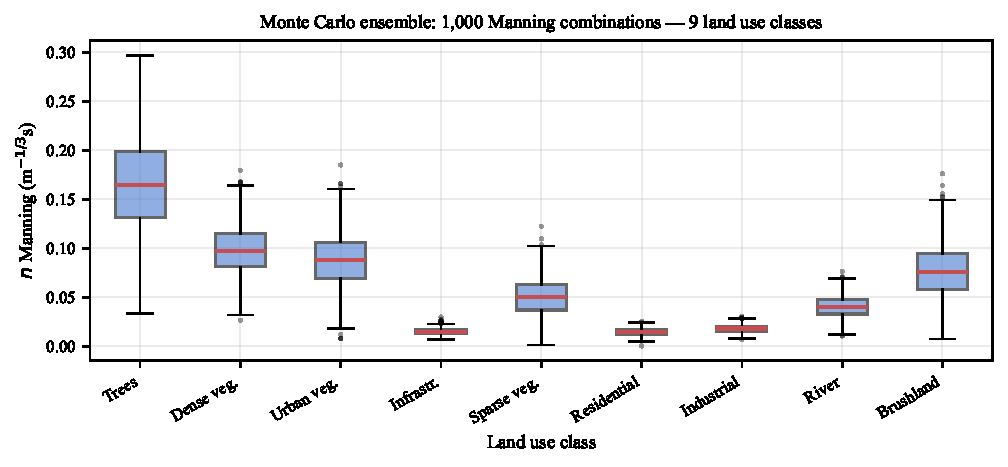
\includegraphics[width=\textwidth]{figures/besaya_fig02_mc_boxplots.pdf}
    \caption{Distribución de Manning del ensemble por clase de uso.}
    \label{fig:mc_boxplots}
  \end{subfigure}
  \hfill
  \begin{subfigure}[b]{0.48\textwidth}
    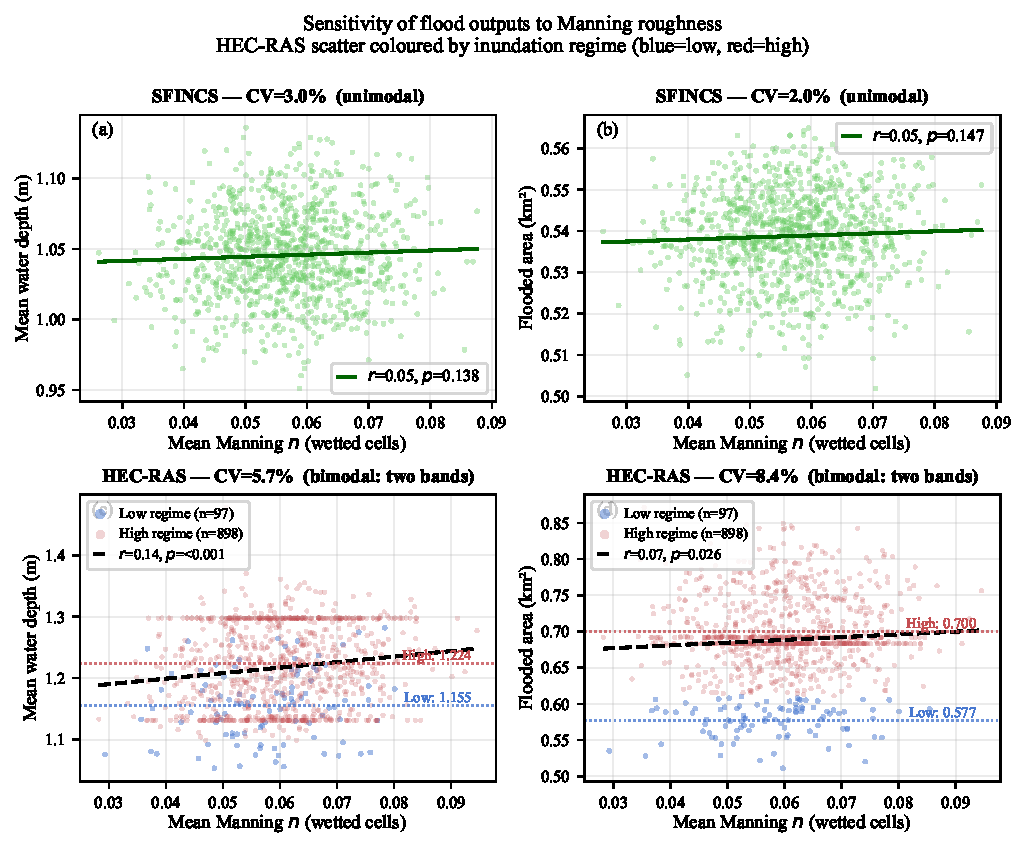
\includegraphics[width=\textwidth]{figures/besaya_fig03_intramodel_sensitivity.pdf}
    \caption{Manning medio frente a calado y área inundada.}
    \label{fig:intramodel}
  \end{subfigure}
  \caption{Ensemble y respuesta hidráulica del análisis de sensibilidad en Los Corrales de Buelna. Izquierda: boxplots de las 1.000 combinaciones de Manning para las nueve clases de uso. Derecha: relación entre Manning medio, calado medio y área inundada para SFINCS y HEC-RAS; las dos bandas de HEC-RAS corresponden a dos regímenes de inundación identificados mediante un modelo de mezcla gaussiana. Fuente: \parencite{navas2025roughness}.}
  \label{fig:sensibilidad_manning}
\end{figure}

\section{Postprocesado y métricas de impacto}

Una vez ejecutados los modelos hidrológicos e hidráulicos, \hydra transforma sus resultados en métricas de impacto comparables entre escenarios. Esta fase es conceptualmente la más importante del flujo: el objetivo final no es producir hidrogramas o mapas de calado, sino cuantificar la probabilidad de superar umbrales de impacto relevantes.

Las métricas disponibles incluyen:
\begin{itemize}
  \item calado máximo por pixel para cada evento o escenario;
  \item velocidad máxima y producto calado-velocidad como indicador de peligrosidad;
  \item extensión inundada sobre un umbral de calado definido por el usuario;
  \item período de retorno por pixel calculado sobre el conjunto de escenarios mediante \texttt{pixel\_return\_period};
  \item hidrograma de caudal punta y volumen de evento en puntos de control.
\end{itemize}

La combinación de estas métricas con los mapas de exposición y vulnerabilidad del territorio permite construir indicadores de riesgo específicos del caso de estudio, cerrando el flujo desde datos climáticos hasta información útil para la toma de decisiones.

El postprocesado mantiene separadas tres capas: salida física del modelo, métrica de impacto y producto de decisión. Un GeoTIFF de calado máximo es una salida física; el período de retorno por pixel es una métrica probabilística; y un mapa clasificado por umbrales de afección es un producto de decisión. Separar estas capas evita confundir el resultado numérico del modelo con la interpretación de riesgo que se realiza posteriormente.
